%#####################################################################
\chapter{関連技術}
%#####################################################################

 本研究では,提案したネットワークモデルをネットワークシミュレータを用いて構築しシミュレーションを行う.
本章では,初めの2.1節で,使用するネットワークシミュレータの説明をする.
2.2節ではSDNおよびOpenFlow技術を説明する.
最後に2.3節では,ネットワークモデルを構築する際に必要となるネットワークの諸技術について説明する.

\section{ネットワークシミュレータ ns-3}

ns-3(Network Simulator Version 3)\cite{ns3} \cite{ns3text} とは,その前身であるns-2の開発に携わっている主要メンバーにより開発された,オープンソースベースの離散イベント駆動型シミュレータである.
% ns-3の開発チームには,Tom Henderson主任研究員を筆頭に,副主任研究員としてSumit Roy(ワシントン大学),George Riley(ジョージア工科大学),Sally Floyd(カリフォルニア大学バークレイ分校ISCIセンター)など,ネットワークの研究分野において著名な研究者たちが名を連ねている.
% 無料で使用可能なシミュレータながら,比較的最近のサービスやプロトコルのサポートを行うなどの積極的な開発を行っている.
ns-3の開発チームには,ネットワークの研究分野において著名な研究者たちが名を連ねておりシミュレータとしての信頼性は高い.
更に,無料で使用可能なシミュレータながら,比較的最近のサービスやプロトコルのサポートを行うなどの積極的な開発を行っている.

ns-3が開発された目的は,有線でのパケット通信しか想定されていなかったり,コードの煩雑・肥大化によるメンテナンスの負担の増加など数々あったns-2の問題点を解消し,ns-2の開発時点では存在しなかった新たなプロトコルの実装および,より大規模なシミュレーションの評価をより簡単にするというものであった.
それに伴い,ns-2でのシナリオを記述する言語として採用していたObject TCL言語の使用を廃止し,事実上C++言語を用いたデザインに統一したため,ns-3とns-2の間の互換性が無くなった.
そのため,長らくは有線ネットワーク系のシミュレーションにはns-2を,無線ネットワーク系および比較的新しい技術を用いたネットワークのシミュレーションにはns-3を使うのが一般的であったが,現在では,ns-2が持っていた機能の移植が着実に進んでおり,徐々にns-3を用いるユーザが多くなっている. \\

ns-3は,本研究で用いるOpenFlow技術に対応済みである他に,以下の機能を備える.

\subsubsection{Pythonによるシナリオファイルの作成}

ns-3では,基本的にC++を用いてコードを記述するが,シミュレートするネットワークモデルの構築を行うシナリオファイルを記述する場合のみ,簡易スクリプト言語であるPythonも使用することができる.
Pythonを用いてシナリオファイルを作成することによって,コード量の削減および可読性が高まるため,結果として第三者が見ても分かりやすいシナリオファイルを作成することができる.

本研究では,ns-3がOpenFlowのPythonバインディングに対応していないということと,Pythonの弱点である実行速度の遅さが如実に表れる可能性があるということから,C++言語を用いてシナリオファイルを作成している.

\subsubsection{tcpdumpを用いたトレースファイルの解析}

シナリオファイルを記述するときに,トレースファイルの生成を可能にするコードを追加することで,パケットキャプチャ用ライブラリのlibpcap形式(以下,PCAP形式)のトレースファイルを生成することができる.
このトレースファイルには,シナリオに登場するノードの全ネットワークデバイスに対し,パケットの入出力データが記されている.
このトレースファイルは,Linuxに標準搭載されているキャプチャツールであるtcpdumpを用いて解析することができ,ネットワークの全体像を把握することが可能になる.

\subsubsection{シミュレーション結果の可視化}

ns-3では,PyVizというライブラリを用いることによって,トレースファイルを用いたシミュレーション結果のアニメーション表示が可能になる.
PyVizは最新のns-3パッケージに標準搭載されているため,特別な導入操作などは不要である.
パケットの通信経路,転送速度などを可視化して表示することができ,シミュレーション結果の時間的な流れを柔軟に変更させながら,結果の解析を行うことができる.

\subsubsection{実機を用いたシミュレーション}

ns-3は,LinuxなどのUNIX系OSに搭載されているTAPデバイスを用いて,現実で動作するホストやデバイスなどをシミュレーション内に統合することができる.
これを用いることで,実際に稼働している通信の一部をシミュレータ内に引き込んでシミュレーションを行うことが可能になるほか,ns-3外でインストールしたソフトウェアと接続してシミュレーションを行うことが可能になる.

\section{SDNとOpenFlow}

本節では,ネットワークモデルを構築する際に採用した技術であるSDNおよびOpenFlow技術について説明する.
OpenFlow技術に関しては,本研究で活用したOpenFlowの仕様も併せて説明する.

\subsection{SDN}

従来のネットワークは,スイッチおよびルータが自律的にネットワークの情報を収集し,その情報に応じてパケット通信を行ってきた\cite{openflownet}.
そのため,ネットワーク管理者が制御できる部分はあまりに限定的であり,ユーザのニーズの多様化に対応できないなどの課題があった.
更に,従来のネットワークは大部分の構成が静的であるという前提の上で,ネットワークの構築を行っていたため,構成を何らかの事情で変更しなければならないとき,従来の方法ではほぼ全てを手作業で変更する必要があり,非常に苦労するものであった.
このような課題を解決するために,ソフトウェアのように柔軟および動的に,経路情報などのネットワーク機器の制御を行う技術が求められた.
このようにして考えられた技術の総称がSDN(Software Defined Network)である.

SDNは,しばしば「ソフトウェアでプログラムするように自由にネットワークの構成を変更できるようなネットワーク」という意味で用いられ\cite{openflowjapanese},現在ではプログラム自動生成,デバッガなど一般的なソフトウェアと遜色ないような機能を加えることはできないかという議論が行われている.

\subsection{OpenFlow}

OpenFlowとは,SDNを用いた代表的なプロトコルで,ネットワーク機器のハードウェアレベルまでの機能の制御を行うことができる技術である\cite{openflowjapanese}.

OpenFlowを用いることで,ネットワーク管理者自身で柔軟にネットワーク環境を構築し,運用することができる.
これにより,従来は大きな時間と労力をかけなければならないネットワーク環境の変更にも,ソフトウェアのようにコードを変更するだけで,ほぼ全て対応でき,比較的短時間で行うことができるようになる.
更に,OpenFlow対応機器を購入し,自身でプログラムすることによって自由にネットワークを構築するため,運用コストが低いという利点がある.

未だ研究段階で実用・一般化されておらず,目途も明らかになっていないが,日本の企業や大学からもこの技術に関する研究や実装事例が多数報告されており,注目が集まっている技術である.

\subsection{OpenFlowの仕様}

OpenFlowプロトコルは,主にスイッチをどのように振る舞わせるかを規定したもので,コントローラおよびアプリケーションを用いて定義する必要がある.

2008年12月に策定されたOpenFlow Version 0.8.9\cite{openflow} から仕様が一般公開されており,執筆現在の最新バージョンは1.5.1である.
今回使用したOpenFlowモジュールはバージョン0.8.9を用いてモデルを構築するため,以下に述べるOpenFlowの仕様は,バージョン0.8.9に基づくものである.

\subsubsection{マッチフィールド}

OpenFlowで用いるマッチフィールドを表 \ref{tab:2-1}に示す\cite{openflow}.

スイッチが予め空のフローテーブルを保有しており,入力されたパケットがフローテーブル内のフローエントリーのマッチフィールドに合致しなければ,スイッチ自身が未知のパケットと判断し,パケットの制御方法をコントローラに問い合わせる.
スイッチからコントローラに問い合わせが来たとき,コントローラに記述されているアルゴリズムをもとに適切な処理をスイッチに伝える.
コントローラから処理手順を伝えられたスイッチは,自身のフローテーブルに処理を追加した後,そのパケットを手順通りに処理する.

フローテーブル内のフローエントリーのマッチフィールドに完全に合致したパケットであれば,スイッチはコントローラに問い合わせることなく,自律的にフローエントリーに基づいてパケットの処理を行う.
マッチングする際に,ワイルドカードを用いることも可能である.

\begin{table}[tb]
	\begin{center}
		\caption{OpenFlowで用いるマッチフィールド}
		\begin{tabular}{c|c}
			\hline
			フィールド & 内容 \\ \hline \hline
			Ingress Port & 受信物理ポート \\ \hline
			Ethernet source address & 送信元MACアドレス \\ \hline
			Ethernet destination address & 宛先MACアドレス \\ \hline
			Ethernet type & パケットのプロトコルタイプ \\ \hline
			VLAN id & VLAN ID(Ethernet typeが0x8100のみ) \\ \hline
			IP source address & 送信元IPアドレス \\ \hline
			IP destination address & 宛先IPアドレス \\ \hline
			IP protocol & TCP/IPのプロトコル番号 \\ \hline
			Transport source port & 送信元のポート番号 \\ \hline
			Transport destination port & 宛先のポート番号\\ \hline
		\end{tabular}
		\label{tab:2-1}
	\end{center}
\end{table}

\subsubsection{アクション}

マッチフィールドを用いてマッチングされたパケットの処理を以下の4つから決定する\cite{openflowjapanese}.
4つの処理の中から複数選択することが可能であり,基本的にはパケットの破棄を除く3つを自由に組み合わせてパケットの処理を行う.

\begin{itemize}
	\item パケット転送
	\item パケットヘッダの変更
	\item パケットのエンキュー
	\item パケットの破棄
\end{itemize}

パケット転送は,入力されたパケットを指定の物理ポートへ転送する処理である.
このとき,物理ポートを指定するほかに,OpenFlowに用意された仮想ポートを指定することができる.
仮想ポートを指定した場合,表 \ref{tab:2-2}にある内容に合致した物理ポートからパケットが出力される.

\begin{table}[tb]
	\begin{center}
		\caption{パケット転送で使用できる代表的な仮想ポート}
		\begin{tabular}{c|c}
			\hline
			仮想ポート名 & 内容 \\ \hline \hline
			OFPP\_ALL & 全ての物理ポートへ転送 \\
			 & (入力ポートを除く) \\ \hline
			OFPP\_CONTROLLER & コントローラへ転送 \\ \hline
			OFPP\_IN\_PORT & 入力ポートへ転送 \\ \hline
			OFPP\_NORMAL & 通常のスイッチと同じ振る舞い \\ \hline
			OFPP\_FLOOD & 全ての物理ポートへ転送 \\
			 & (入力ポートおよび規制されたポートを除く) \\ \hline
		\end{tabular}
		\label{tab:2-2}
	\end{center}
\end{table}

パケットヘッダの変更は,入力されたパケットのヘッダフィールドを変更する処理である.
この処理を行った場合,各フレームのチェックサムも同時に再計算され変更される.
変更可能なヘッダフィールドの処理を以下に示す.

\begin{itemize}
	\item VLAN IDの変更
	\item VLAN優先度の変更
	\item VLANタグの除去(タグVLAN使用時のみ)
	\item 送信元MAC addressの変更
	\item 宛先MAC addressの変更
	\item 送信元IP addressの変更
	\item 宛先IP addressの変更
	\item パケット処理の優先度を示すToSフィールドの変更
	\item 送信元のポート番号の変更
	\item 宛先のポート番号の変更
\end{itemize}

パケットのエンキューは,OpenFlowスイッチ内にキューを持つとき,それぞれの物理ポートの持つキューにパケットを入れる処理である.

パケットの破棄は,フローエントリーは存在するが転送処理が規定されていない場合はそのパケットを破棄するという仕様を利用して,作為的に空のフローエントリーを作成することで実現できる.

\section{ネットワークモデル構築に必要な諸技術}

本節では,ネットワークモデルを構築する際に必要となる諸技術について説明する.

\subsection{MACアドレス}

MACアドレスとは,データリンクに接続されているノードを識別するためにIEEEが規格化した48ビットで構成されているユニークなアドレスである\cite{masteringtcpip}.
一般的なコンピュータに搭載されているNIC(ネットワーク・インタフェース・カード)の場合はマザーボードなどに焼きこまれており,このときにMACアドレスのユニーク性を保証するように設定される.
MACアドレスは通常「9E-0D-FE-54-A9-F9」や「1D:98:D2:69:EC:76」など,8ビット列の6組に分け16進数表記で記載する.
3~24ビットにはNICのメーカーごとに特定の数字が割り当てられたベンダ識別子が,25~48ビットにはメーカーが製造したNICごとに違う製造番号が割り当てられている.

これにより,ネットワークの異常を検知した際に疑わしいフレームを解析し,MACアドレスを調べることによって,どのメーカーのNICで異常なフレームを送信しているかを特定することができる.
これは,ネットワークがマルチベンダ環境で構築されている場合の原因特定に役立つ場合もある.

このMACアドレスは,データリンクの種類にかかわらずユニークになるように割り当てられるため,イーサネットと無線LAN,Bluetoothなどデータリンクの種類が異なる通信が同じ端末内に存在する場合でも,同じアドレスが割り当てられることはない.

\subsection{IPアドレス}

IPアドレスとは,インターネットにある全てのホストおよびルータが保持しているアドレスである\cite{tanenbaum}.
現在一般的に使用されているIPv4は32ビットで構成されており,IPパケット上で送信元アドレスと宛先アドレスの指定に用いられている.
通常,人間でも認識しやすくするために,「33.205.102.82」というように32ビットを8ビット列の4組に分け,10進数表記で記載する.

IPアドレスはMACアドレスとは異なり,階層構造を持つ\cite{masteringtcpip}.
32ビットのIPアドレスのうち,上位ビットをネットワーク部,下位ビットをホスト部と呼び,ビット長は可変長である.
ネットワーク部はデータリンクのセグメントごとに割り当てられており,全てのセグメントのアドレスと重複しないように設定しなければならない.
このため同じセグメントに接続されているホストは,ネットワーク部のビット列が同じである.
一方,ホスト部は同じセグメント内のホスト同士が重複しないように設定される.
これによりネットワーク全体でユニークなIPアドレスを割り当てることができる.

しかし,ネットワーク部とホスト部は合計32ビットであるという制約のもと,ビット長は可変長であるため,IPアドレスだけではそれぞれのビット長がどれほどかを判断することはできない.
この問題の解決方法は主に2種類ある.

初期の規格では,ネットワーク部とホスト部はクラスA~Dおよび未定義のクラスEによって区別されていた.
これらは表 \ref{tab:2-3}のように各クラスにおいて,使用できるアドレスの範囲,用途を定義している.
しかし,クラスによるネットワーク部とホスト部の区別は融通が利きにくく,上位のクラスをそのまま使うのは無駄などの問題点が指摘されていた.

\begin{table}[tb]
	\begin{center}
		\caption{IPにおけるクラスの特徴}
		\begin{tabular}{c|c|c|c}
			\hline
			クラス名 & ネットワークアドレスの範囲 & ビット長 & 用途 \\ \hline \hline
			クラスA & 0.0.0.0~127.0.0.0 & 8ビット & 大規模ネットワーク\\ \hline
			クラスB & 128.0.0.0~191.255.0.0 & 16ビット & 中規模ネットワーク \\ \hline
			クラスC & 192.0.0.0~223.255.255.0 & 24ビット & 小規模ネットワーク \\ \hline
			クラスD & 224.0.0.0~239.255.255.255 & 32ビット & IPマルチキャスト通信\\ \hline
			クラスE & & & 実験用 \\ \hline
		\end{tabular}
		\label{tab:2-3}
	\end{center}
\end{table}

現在の規格では,クラスの考え方を継承し,以前の問題点を縮小したサブネットマスクにより区別している.
つまり,現在はIPアドレスを通常のアドレスとサブネットマスクの2種類の識別子で表すようになった.

サブネットマスクは,IPアドレスと同じく32ビットで,IPアドレスのネットワーク部を表すビットを全て1に,ホスト部を表すビットを全て0にして表記する.
例えば,IPアドレスの上位25ビットがネットワーク部であった場合,サブネットマスクの上位25ビットを1に,下位7ビットを0にした「255.255.255.128」がサブネットマスクということになる.
これにより,ネットワーク部のビット長をクラスに縛られることなく柔軟に変更することができるようになった.

\subsection{L2スイッチ}

L2スイッチとは,同一ネットワーク内でブリッジの役割を持つネットワークデバイスのことであり,基本的にレイヤ2の情報を用いて処理を行う\cite{masteringtcpip}.
ホストからL2スイッチに送られたフレームは,L2スイッチ内によってそのフレームの宛先MACアドレスを解析され,どの物理ポートから転送されるかが決定される.
このとき,L2スイッチ内では転送ポート決定の際に,MACアドレスと接続物理ポートの組を記したテーブルを参照する.
これを転送表(フォワーディングテーブル)と呼び,全てのL2スイッチが個々に保持する.

一般的なL2スイッチは,パケットを受け取った際に,送信元MACアドレスと入力物理ポートの組を転送表に記録する.
なぜならば,あるMACアドレスAが送信元のフレームを物理ポートBで受け取ったということは,その物理ポートBの先にMACアドレスAを持つホストが存在していることを意味し,今後そのMACアドレスAが宛先の場合,物理ポートBから転送すれば,確実にMACアドレスAのホストに到達すると考えてもよいからである.
この考え方に基づいた転送表の記録を自己学習といい,この自己学習を積み重ねることによってL2スイッチはインテリジェントなものになる.
もし,宛先MACアドレスが転送表にない場合は,入力ポート以外の全ての物理ポートに転送するフラッディング動作を行い,他のネットワーク機器からの応答を待つ.

\subsection{侵入検知システムと侵入防御システム}

ネットワークを脅威から守る方法は様々あるが,そのほとんどがファイアウォールのようにネットワーク外部からの脅威の侵入に対する防御にしか対応ができない.
更に,このような装置の場合,パケットの内容まで監視しているわけではないため,不正な侵入を完全に防ぐことは難しい.
そのため,一般的に情報セキュリティの世界では侵入検知システムおよび侵入防御システムを併用する.

侵入検知システム(Intrusion Detection System; IDS)とは,ネットワークを流れるパケットを監視し,サーバ上でデータを解析しながら不正な侵入を検知するものである\cite{idsandips}.
IDSはファイアウォールなどと違い,パケットの内容まで解析して判断する.
そのため,通信を行ったパケットが不正なパケットなのかをより精密に判定することができる.
しかし,IDSはその名の通り,不正な侵入を検知するだけの機器のため,システム自体がネットワークに対し処理を行うわけではなく,不正な侵入があったという事実をネットワーク管理者に通報するのみである.
これにより,通報を受けた管理者が不正な侵入に対応するには一定の時間がかかり,その間に被害が拡大する可能性がある.
そのため現在では,このシステムを改良した侵入防御システムを用いることが増えてきた.

侵入防御システム(Intrusion Prevention System; IPS)とは,IDSに不正な通信を自動的に遮断する機能を追加したシステムである.
これにより,不正なパケットをシステムが検知してからネットワークを保護するまでの時間をほぼゼロにすることが可能になり,ネットワーク内に大きな打撃を与えずに済むことができる.

一般的なIPSはその設置方法により,2つの接続形態で動作させることが可能である.

\subsubsection{プロミスキャスモード}

プロミスキャスモードとは,図 \ref{fig:2-1}のようにネットワークの構造の外側に設置するタイプで,ある監視対象のノードを設定し,そのノードを通過する全ての通信をミラーポートからIPSに転送させ検査する\cite{ciscoips}.
このとき,IPSが不正な通信だと判断した場合,監視対象のノードに不正な通信を遮断するようにアクションを送る.

\begin{figure}[tb]
	\begin{center}
		\scalebox{0.5}{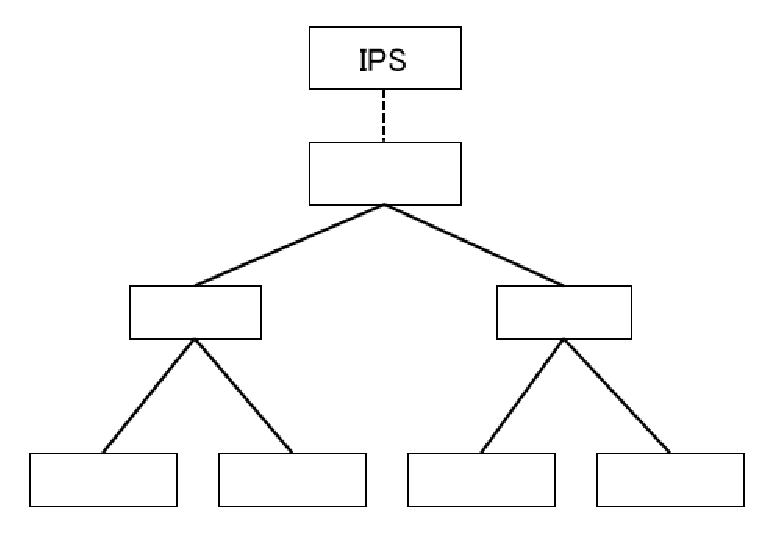
\includegraphics{./img/eps/2-1.eps}} 
		\caption{プロミスキャスモード}
		\label{fig:2-1}
	\end{center}
\end{figure}

IPSを直接パケットが通るわけではないため,通信トラフィックに影響を与えることなく検査することが可能である.
更に,プロミスキャスモードでの検査の場合,IDSを用いても一定の成果を上げることができるため,ほぼ全てのIDSおよびIPSを用いて検査をすることが可能となり,機器の選択の幅も広がる.

しかし,IPSが直接ネットワーク内に介入し検査を行うわけではないため,通信遮断のアクションがノードに伝わるまでに一定の時間が必要となる.
このため,その間にいくつかの不正なパケットがノードを通過する可能性がある.
更に,ノードを通過してから検査をして次のパケットから対策するという手法のため,攻撃がシングルパケットで収束してしまうようなアトミック攻撃には対応が難しく,被害が及んでしまう可能性もある.
そのため,脅威に関する防御能力は高くなく,IPSを用いての検査では推奨されない.

\subsubsection{インラインモード}

インラインモードとは,図 \ref{fig:2-2}のようにネットワークの構造にIPSが直接組み込まれ,パケットがIPS本体を通過することで検査するタイプである\cite{ciscoips}.
このとき,IPSが不正な通信だと判断した場合,IPS機の中でパケットをドロップし,セッションを強制的に終了させる.

\begin{figure}[tb]
	\begin{center}
		\scalebox{0.5}{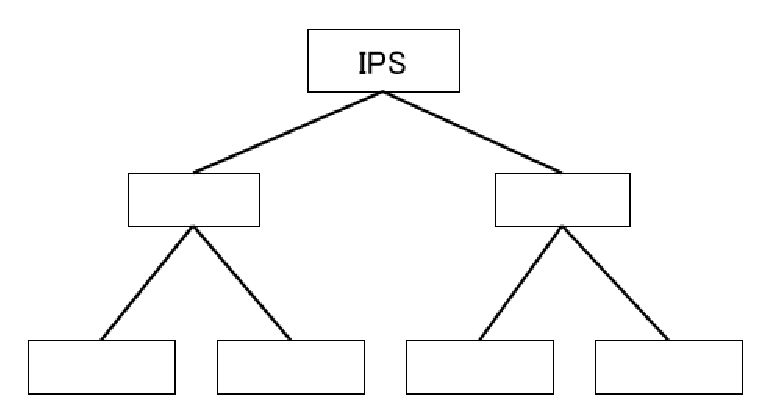
\includegraphics{./img/eps/2-2.eps}} 
		\caption{インラインモード}
		\label{fig:2-2}
	\end{center}
\end{figure}

インラインモードでの検査の場合,より高度な埋め込み攻撃にも対応するために,ほぼ全てのレイヤの内容について解析する.
これにより,精度の高い判断ができるため,ファイアウォールなどを通過した攻撃を阻止することができる.
更に,IPSが問題なしと判断しないとパケットが送り出されない仕組みのため,プロミスキャスモードでは防ぐことができなかったアトミック攻撃にも対応することができる.

しかし,IPSが通過するトラフィックを全て検査するため,IPSの性能によってネットワーク全体の性能が大きく左右される.
もし一定規模のネットワークの内部をIPSを用いて検査しようとする場合,そのトラフィック量はネットワーク外部とのトラフィック量とは比較にならず,中途半端な性能の製品を導入すると全体の転送速度が大きく低下する危険性がある.